\section{Experiments} % (fold)
\label{cha:experimental_setup}
\todo[inline]{Don't forget to cover details like sampling method, features (separate subsection?), difference in settings for each test and data set, etc.

ALSO: INCLUDE RESULTS!}

The previously elaborated theory on local NBNN exemplar model detection was tested in a number of experiments. First, the NBNN detection experiments of Becker \cite{becker2012codebook} were replicated to validate the implementation, see Section~\ref{sec:nbnn_detection}. These experiments were altered in a number of ways, to see the effects of different descriptors, feature selection rules, clustering algorithms and using Behmo's optimized NBNN approach. In the final experiment, McCann's Local NBNN was integrated into the detection algorithm (Section~\ref{sec:local_nbnn_detection}). Most tests were performed on both the TUDmotorbikes and VOC2007 benchmark detection sets.

\subsection{Features} % (fold)
\label{sec:features}

In most experiments, feature selection is done by dense sampling. Each point was sampled at various scales, to allow for scale invariance. The basic feature that has been used was the scale-invariant feature transform (SIFT). \cite{lowe2004distinctive}

\todo[inline]{Is it necessary to include rootsift/colorsift? No good results obtained with it}

% section features (end)

\subsection{PASCAL VOC Data Set} % (fold)

\label{sec:voc_data_set}
The Visual Object Classes (VOC) 2007 challenge of the PASCAL network \cite{pascal-voc-2007} provides a data set annotated for image detection. The data set consists of 20 object classes plus a background class, on a total of 9,963 images containing 24,640 annotated objects. The images are all taken from Flicker, and show a large variety of image quality and a large intra-class variety of objects. The data set is subdivided into 50\% test set, 25\% training set and 25\% validation set, with approximately equal distribution of class object distribution over the sets.

The VOC 2007 dataset is partly annotated for class segmentation, 844 images subdivided in the same way as the full set. This subset is used for the experiments below, in part because segmentation proved to be a good ground truth for descriptor selection, and also because of time and memory constrains both for training and testing the algorithms.

% section voc_data_set (end)

\subsection{TUD motorbikes Data Set} % (fold)
\label{sec:tudmotorbikes_data_set}
The TUD Motorbikes data set is a selection of motorbikes from different benchmark sets. \cite{fritz2005integrating} The training set consists of 153 images of motorbikes to a uniform background, and are segmented into motorbike and background. The test set consists of 115 images, all of motorbikes, with various backgrounds. Becker \emph{et al.} \cite{becker2012codebook} use this benchmark to test their setup. In the training phase they train on the motorbike features from the TUD train set, and randomly add features from non-object areas of the PASCAL VOC 2007 set, as background features. This same setup was used as a comparison to Becker's experiments.

% section tudmotorbikes_data_set (end)


% SKIP THIS PART
% \subsection{NBNN Classification} % (fold)
% \label{sec:nbnn-cls}
% \todo[inline,color=red]{This section only if the tests succeed. Most of the method is already in the NBNN section.}
% 
% % section nbnn-cls (end)

\subsection{Exemplar-NBNN Detection} % (fold)
\label{sec:nbnn_detection}

The first experiment is used to verify the results of Becker \emph{et al.} \cite{becker2012codebook}. In addition to this, some parameters of this approach were altered to see what effects they have on the overall performance.

This experiment was performed on the TUD Motorbike set in the setup used by Becker (c.f. Section~\ref{sec:tudmotorbikes_data_set}). The SIFT descriptors were collected using dense sampling, using a step size of 8 pixels, and patch sizes of $32\times32$, $48\times48$ and $64\times64$. I repeated each test 5 times with a different random selection of background images from the VOC 2007 data set, to avoid possible artifacts. FLANN was used to perform approximate NN, using the kd-tree algorithm with 4 trees and 1000 checks to assure high enough accuracy.

The similarity measure between hypotheses, used as a basis for the clustering algorithm, was defined as the area of overlap ($AO$) between two hypotheses:
\begin{equation}
    AO(H_a, H_b)= \frac{|H_a\cap H_b|}{|H_a\cup H_b|}
\end{equation}

Clustering was done using the single-link agglomerative clustering algorithm (Section~\ref{sub:agglomerative_clustering}), using 2 parameters: $\theta_m$, which defines the minimal overlap between hypotheses to be clustered together, and the maximal overlap between detections: $\theta_p$. I set the parameters such that $\theta_m = 0.8$ and $\theta_p = 0$, conform to Becker.

Detections were ranked according to their ``detection quality'', $Q_D$. This measure is defined as the amount of hypotheses being clustered into one detection. Ties being broken by a second ordering, called ``hypothesis quality'', $Q_H$, which is defined as the distance of a hypothesis to the foreground class, relative to its distance to the background class: $\frac{d_{bg} - d_{fg}}{d_{fg}}$. 

Performance was measured with the average precision (AP) of the ranked detections, and visualized in a precision-recall curve.

\subsubsection{NBNN Detection Using Quickshift clustering} % (fold)
\label{sub:nbnn_detection_using_quickshift_clustering}

\todo[inline]{Write a short piece on quick shift clustering, the parameters and stuff}

I compared the results of detection using single link clustering with quickshift clustering. Because quickshift is a mode finding algorithm, it is guaranteed to find local maxima in the hypothesis density space. Therefore, it gives a more theoretically sound basis for clustering hypotheses, perhaps improving results along the way. Quickshift has one parameter, $\tau$. This represents the expected variance within the clustering space, and defines the maximal variance to be clustered, somewhat like $\theta_m$ in single link clustering.

Quickshift has no bound for overlap in detections, which should not be a problem as the test images might have multiple overlapping objects. To make this comparison fair towards single link clustering, I varied the value of $\theta_p$ in the latter algorithm. For quickshift I settled on $\tau = 1.2$, for single link clustering $\theta_p = 0.4$ seemed ideal.

% subsection nbnn_detection_using_quickshift_clustering (end)
\subsubsection{Training Weighted Distances} % (fold)
\label{ssub:training_weighted_distances}

In image classification, the classes are generally quite well balanced. The amount of images in every class is usually approximately the same and all image are usually of the same size, making the assumption of a uniform prior hold. Therefore the natural distribution of descriptors in feature-space can be assumed to be equally sampled in every class. This makes it acceptable to use a learning method like optimal NBNN \cite{behmo2010towards} to tune the likelihood of classes to the local density in feature space to be equal for all classes.

In object detection, the sampling rate will not be equal over classes, especially the background class will have a larger sampling rate, simply because it will occur in virtually all images. The equal priors assumption therefore does not hold. This flaw is mitigated by the fact that a higher number of sampled descriptors also tends to make the feature space for that class more dense, and more likely to be the nearest neighbor.

The risk however is that the estimation of the feature space may differ largely per class. Classes with a large intra-class variety of descriptors, but with generally small objects will be sampled much sparser than classes with less descriptor variety and larger objects. Learning parameters to tune the feature space density might therefore result in overfitting for sparsely sampled classes or classes with a very high intra-class diversity.

This experiment will test this hypothesis using Behmo's optimal NBNN linear program to train per-class parameters on sampled images.

\todo[inline]{more detail about implementation of Behmo. Perhaps put the first part either to conclusion, or to theory?}

% subsubsection training_weighted_distances (end)

\subsubsection{Exemplar-NBNN Results} % (fold)
\label{sub:exemplar_nbnn_results}
\todo[inline]{Behmo results??}

Figure~\ref{fig:tudk1clusteralgos} shows the results of my implementation of Becker's algorithm using Single-link clustering, compared to the quickshift algorithm. Single-link clustering with $theta_p = 0.4$, instead of Becker's $0.0$ was also added. It shows that quickshift performs better than single-link clustering.

\begin{figure}[hbt]
    \centering
    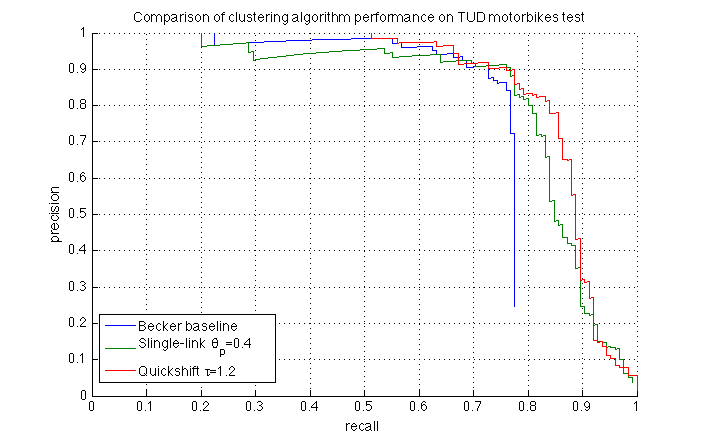
\includegraphics[width=0.8\textwidth]{TUD_k1_clusteralgs}
    \caption{Precision-Recall curves of the TUD Motorbikes detection task, using Becker's \cite{becker2012codebook} setup as baseline, Single-link clustering with a maximal detection overlap of 0.4 and quickshift clustering with $\tau = 1.2$.}
    \label{fig:tudk1clusteralgos}
\end{figure}

\begin{table}
    \caption{Comparison of test statistics of TUD Motorbikes tests using various clustering algorithms and settings. \emph{Baseline} represents the result reported by Becker \cite{becker2012codebook}.}
    \label{tab:tudk1clusteralgos}
    \begin{tabular}{rc|cc>{\bfseries}c}
        ~&k&no. of detections&total recall&average precision \\
        baseline & 1 & --- & --- & 0.83 \\
        Becker's settings & 1 & 394 & 0.7760 & 0.7536\\
        single-link $\theta_P=0.4$ & 1 & 3447 & 0.9920 & 0.8342\\
        quickshift $\tau=1.2$ & 1 & 7968 & 1.0000 & 0.8680\\
        quickshift $\tau=1.2$ & 4 & 8147 & 0.9680 & 0.8940\\
        single-link $\theta_P=0.4$ & 20 & 3713 & 0.9920 & 0.8491\\
        quickshift $\tau=1.2$ & local,4 & 12406 & 0.9520 & 0.8169
    \end{tabular}

\end{table}

Table~\ref{tab:tudk1clusteralgos} shows some more statistics of the experiments. The results reported by Becker are somewhat higher than my own replication. This might be caused by a fortunate set of random background descriptors. Becker does not report the randomization process involved, so I was not able to replicate the results exactly. It also clearly shows that raising the $\theta_P$ threshold for the maximal overlap between detections should not be 0, because the recall gets much higher when it is set higher.


\todo[inline]{Results on VOC07?}

\begin{figure}[hbt]
    \centering
    \missingfigure[figwidth=0.8\textwidth]{Result graph VOC07}
\end{figure}


\begin{table}[hbt]
    \centering
    \missingfigure[figwidth=0.8\textwidth]{Result table VOC07}
\end{table}
% subsection exemplar_nbnn_results (end)

% section nbnn_detection (end)

\subsection{Exemplar-$k$NBNN Detection} % (fold)
\label{sec:local_nbnn_detection}
A downside of the exemplar-NBNN method is the descriptor aliasing problem explained in Section~\ref{sec:descriptor_aliasing}. This can be solved by taking the $k$ of $k$NN to be greater than 1. This means that the $k$ closest neighbors over all classes (the object class and the background class) are taken into account when constructing detection hypotheses. Within these $k$ nearest neighbors, the ones belonging to the object class that are closer than any neighbor in the background class, are transformed into detection hypotheses. This $k$NBNN approach was tested in the detection algorithm and compared to the previous setup.

\subsubsection{Local NBNN Detection} % (fold)
\label{ssub:local_nbnn_detection}

Another disadvantage of exemplar-NBNN detection is it returning many false positive detections for images not having any objects of the current object class. The reason for this is obvious, as all descriptors closer to the class than to the background will be regarded as hypotheses, and therefore images without any objects get reasonably well ranked detections. This problem gets larger as the data sets contains more object classes.

A solution for this is to not only compare the current object class with the background class, but to compare it with all other classes, to see what each descriptor in the test image looks most like. This results in a hypothesis selection step that chooses only descriptors that are closer to the current class than to any other.

This however would create another problem not present in the original approach. Some descriptors could be an indication for multiple classes, because certain parts of objects are quite similar. While the original exemplar-NBNN approach allows for this, regarding each class independently, this multi-class approach prevents this. Think of the similarity of a bicycle wheel with that of a motorbike or a car. To disregard all but one of these classes might cause very little evidence for most classes in an image, giving less stable detections. This reminds of Boiman's argument that much evidence is vital for the NBNN method, because the Naive Bayes assumption is only met towards infinity and there is no training phase to compensate for it.\cite{boiman2008defense}

At the same time, the goal to compare all classes simultaneously is similar to McCann's formulation of local NBNN's query.\cite{mccann2012local} (\emph{cf.} Section~\ref{sec:local_nbnn}). Merging all class indexes into one, and taking into account not only the first NN per class, but the $k$ NN \emph{overall} prevents having too many false positive results, while keeping the possibility of a descriptor to be used for a hypothesis for multiple classes like in the original problem.

As a bonus, local NBNN for detection also incorporates a way to prevent the aliasing problem. Among the $k$ closest neighbors, there might be multiple ones from the same class. Instead of disregarding these neighbors like local NBNN does, they can be taken into account by creating hypotheses for all non-background nearest neighbors.

% subsubsection local_nbnn_detection (end)

\subsubsection{LNBNN Results} % (fold)
\label{ssub:lnbnn_results}
\todo[inline]{Results of kNBNN, localNBNN both TUD motorbike and VOC07}

As shown in Figure~\ref{fig:tudlocalprecrec}, Performance on the TUD Motorbikes task improves the results with quickshift even further. The optimum appeared to lie at $k=4$, while the optimum for single-link runs was at $k=20$. Interestingly, LNBNN seems to perform worse than regular $k$NBNN. This might be due to the task, having only one class and all test images containing at least one motorbike.

On VOC 2007 test, performances are much lower overall. This test however shows more of the differences between methods (Figure~\ref{fig:voclocalaps} and Table~\ref{tab:voclocalaps}). It shows that the methods can keep up fairly well with the state of the art results of the VOC 2007 detection challenge \cite{pascal-voc-2007}, but that there is much variance between classes, both in absolute performance and relative to the baseline. Take in mind that I trained on a subset of the available training images only, and I tested on a subset of the test set too. It would be interesting to see results on the full train and test set, even though much of the train set was not segmented and therefore not available for comparison, and the time for detection of a single image was prohibitive for testing the full test set.
\todo[inline]{In the Analysis, give more explanation on time/memory constraints as a big downside of the method}

Interestingly, using Harris-Laplacian interest point detection instead of dense sampling does not make the performance significantly worse, while speeding up the process significantly.

\begin{figure}[hbt]
    \centering
    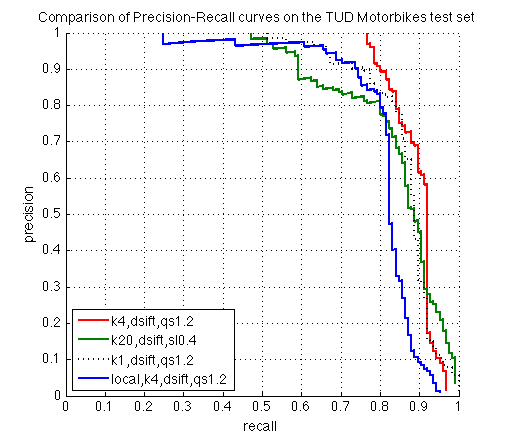
\includegraphics[width=0.8\textwidth]{TUD_local}
    \caption{Precision-Recall curves of the TUD Motorbikes detection task for various tasks using $k>1$, with the best performing $k=1$ result as reference.}
    \label{fig:tudlocalprecrec}
\end{figure}
\todo[inline]{perhaps plot bars of median AP for all classes per method, might be (more) insightful (used by VOC)}
\begin{figure}[hbt]
    \centering
    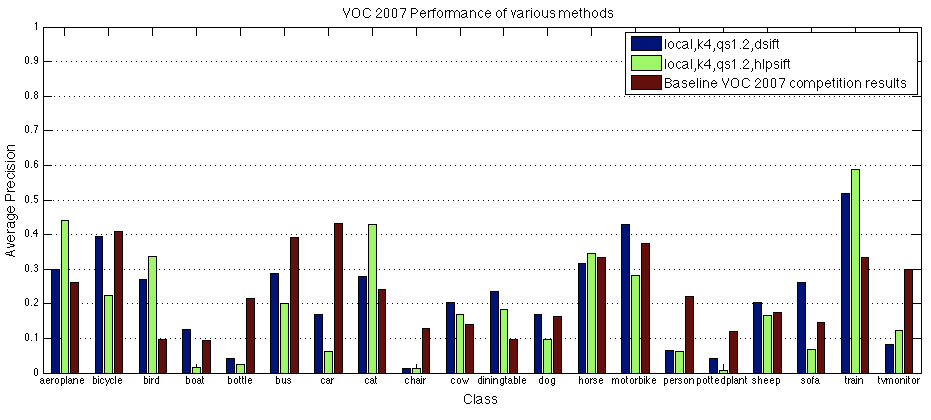
\includegraphics[width=0.8\textwidth]{VOC_aps}
    \caption{Average precision on the VOC 2007 task, for all classes. Blue: Settings with highest performance on the TUD Motorbikes test. Green: Selection of descriptors using Harris-Laplacian instead of dense sampling. Red: Best scores on the VOC 2007 Detection Challenge \cite{pascal-voc-2007}.}
    \label{fig:voclocalaps}
\end{figure}

\begin{table}[hbt]
    \centering
    \caption{Comparison of Average Precision on the VOC 2007 test, for local NBNN and a baseline of the best performances achieved in the VOC 2007 challenge.}
    \label{tab:voclocalaps}
    \begin{tabular}{rccc}
    class & local,k=4,densesift,qs1.2 & local,k=4,hlpsift,qs1.2 & VOC07baseline\\
    \hline
    aeroplane &       0.2982 & \underline{0.4399} & 0.2620\\
    bicycle &         0.3959 & 0.2253 & \underline{0.4090}\\
    bird &            0.2700 & \underline{0.3368} & 0.0980\\
    boat &            \underline{0.1258} & 0.0166 & 0.0940\\
    bottle &          0.0410 & 0.0248 & \underline{0.2140}\\
    bus &             0.2877 & 0.2007 & \underline{0.3930}\\
    car &             0.1701 & 0.0614 & \underline{0.4320}\\
    cat &             0.2787 & \underline{0.4298} & 0.2400\\
    chair &           0.0120 & 0.0129 & \underline{0.1280}\\
    cow &             \underline{0.2036} & 0.1689 & 0.1400\\
    diningtable &     \underline{0.2352} & 0.1844 & 0.0980\\
    dog &             \underline{0.1677} & 0.0964 & 0.1620\\
    horse &           0.3167 & \underline{0.3467} & 0.3350\\
    motorbike &       \underline{0.4284} & 0.2810 & 0.3750\\
    person &          0.0644 & 0.0622 & \underline{0.2210}\\
    pottedplant &     0.0408 & 0.0086 & \underline{0.1200}\\
    sheep &           \underline{0.2031} & 0.1655 & 0.1750\\
    sofa &            \underline{0.2619} & 0.0681 & 0.1470\\
    train &           0.5187 & \underline{0.5874} & 0.3340\\
    tvmonitor &       0.0835 & 0.1230 & \underline{0.2980}
    \end{tabular}

\end{table}

\begin{figure}
    \centering
    \missingfigure{Comparison of test times}
\end{figure}

% subsubsection lnbnn_results (end)
% section local_nbnn_detection (end)
% chapter experimental_setup (end)